\documentclass{article}
\usepackage[utf8]{inputenc}
\usepackage{graphicx}
\usepackage{ragged2e}
\usepackage[margin=2.5cm]{geometry}
\usepackage{array}
\usepackage{wrapfig}
\usepackage{multirow}
\usepackage{tabularx}
\usepackage{amsmath}
\usepackage{wrapfig}
\usepackage{mathtools}
\usepackage[table]{xcolor}
\usepackage{multirow}
\usepackage{polski}
\usepackage{rotating}


\title{Model zbiorników}
\author{Marcin Gruchała 248982\\
Jan Bronicki 249011\\}
\date{}

\begin{document}

\maketitle

\section{Cel sprawozdania.}
Badanie liniowych i nieliniowych modeli kaskady niewspółdziałającej.
\section{Opis modelu.}
W ćwiczeniu badamy kaskadę niewspółdziałającą przedstawioną poniżej:

\begin{figure}[h]
    \centering
    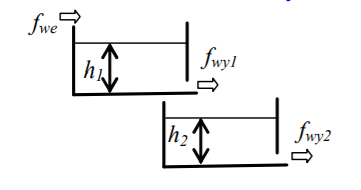
\includegraphics{obrazek_zbiornikow.png}
    \label{fig:my_label}
\end{figure}
$$
\begin{cases}
    A_1\dot h_{1}(t)=f_{we}(t)-A_{w1}\sqrt{2gh_1(t)}\\
    A_2\dot h_{2}(t)=A_{w1}\sqrt{2gh_1(t)}-A_{w2}\sqrt{2gh_2(t)}
  \end{cases}
$$
$$
f_{wy1}(t)=A_{w1}\sqrt{2gh_1(t)}
$$
$$
f_{wy2}(t)=A_{w1}\sqrt{2gh_2(t)}
$$

\begin{flushleft}
gdzie:
\end{flushleft}
$ A_1, A_2 $ - szerokość zbiorników 1 i 2\\
$Aw_1, Aw_2$ - wielkość otworów w zbiornikach przez które wypływa woda\\
$h_1, h_2$ - wysokość słupa wody w zbiorniku 1 i 2\\
$h_{max}$ - maksymalny poziom wody \\
$fwe, fwe_{max}$ - wpływ wody do zbiornika oraz jego maksymalna wartość\\
$f_{wy1}, f_{wy2}$ - wypływ wody ze zbiornkó 1 i 2 \\
W ćwiczeniu oba zbiorniki mają take samw wymiary.


\section{Model nieliniowy.}
Model nieliniowy opisują równania:
$$
  \begin{cases}
    A_1\dot h_{1}(t)=f_{we}(t)-A_{w1}\sqrt{2gh_1(t)}\\
    A_2\dot h_{2}(t)=A_{w1}\sqrt{2gh_1(t)}-A_{w2}\sqrt{2gh_2(t)}
  \end{cases}
$$
$$
  \begin{cases}
    \dot h_{1}(t)=\frac{1}{A_1} \left(f_{we}(t)-A_{w1}\sqrt{2gh_1(t)}\right)\\
    \dot h_{2}(t)= \frac{1}{A_{2}} \left( A_{w1}\sqrt{2gh_1(t)}-A_{w2}\sqrt{2gh_2(t)}\right)
  \end{cases}
$$
Parametry zbiorników:\\             
$A_1$ = 4 \\
$A_2$ = 4  \\
$Aw_1$ = 4  \\
$Aw_2$ = 4\\
$h_{max}$= 6 \\
$fwe_{max}=A_{w1}\sqrt{2gh_{max}}$\\\\
Warunki początkowe dla $h_1(0)$ i $h_2(0)$ można obliczyć z równania statycznego:
$$
\begin{cases}
    0=f_{we}-A_{w1}\sqrt{2gh_1(0)}\\
    0=A_{w1}\sqrt{2gh_1(0)}-A_{w2}\sqrt{2gh_2(0)}
 \end{cases}
 $$
 Dla $h_1(0):$
 $$
    f_{we}=A_{w1}\sqrt{2gh_1(0)}
 $$
 $$
 h_1(0)=\frac{{f_{we}}^2}{{A_{w1}}^22 g}
 $$
 Dla $h_2(0):$
 $$
     A_{w1}\sqrt{2gh_1(0)}=A_{w2}\sqrt{2gh_2(0)}
 $$
 $$
 {A_{w1}}^22gh_1(0)={A_{w2}}^22gh_2(0)
 $$
 $$
 {A_{w1}}^2h_1(0)={A_{w2}}^2h_2(0)
 $$
 $$
 h_2(0)=\frac{{A_{w1}}^2h_1(0)}{{A_{w2}}^2}=
 \frac{{A_{w1}}^2}{{A_{w2}}^2}\cdot\frac{{f_{we}}^2}{{A_{w1}}^22 g}
 $$
 $$
 h_2(0)=\frac{{f_{we}}^2}{{A_{w2}}^22g}
 $$
 


\begin{flushleft}
Schemat:

\end{flushleft}
\begin{figure}[h!]
    \centering
    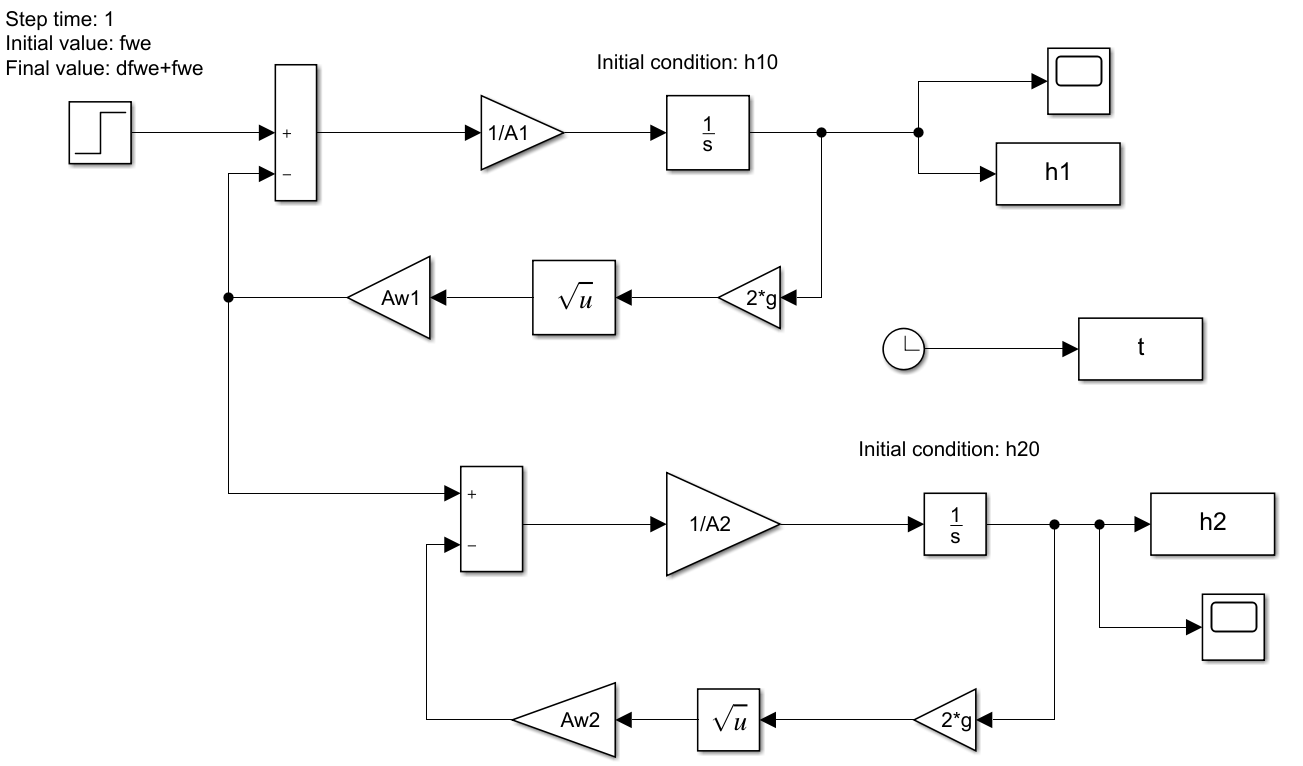
\includegraphics[width=0.955\textwidth]{schematNL.png}
    \label{fig:my_label}
\end{figure}
\section{Model liniowy.}
Model liniowy opisują równania:
$$ 
 \begin{cases}
    A_1\dot h_{1}(t)=f_{we}(t)-a_{1}h_1(t)\\
    A_2\dot h_{2}(t)=a_{1}h_1(t)-a_{2}h_2(t)
  \end{cases}
$$

$$ 
  \begin{cases}
    \dot h_{1}(t)=\frac{1}{A_1} \left(f_{we}(t)-a_{1}h_1(t)\right)\\
    \dot h_{2}(t)= \frac{1}{A_{2}} \left( a_{1}h_1(t)-a_{2}h_2(t)\right)
  \end{cases}
 $$
 Model liniowy polega na uproszczeniu modelu do równania prostej.
 $$
f_{wy}=A_{w}\sqrt{2gh}\approx ah
 $$
 Współczynnik $a$ można obliczyć podstawijąc do równania $fwy_{max}$ i $h_{max}$, wiedząc że $fwy_{max}=A_{w}\sqrt{2gh_{max}}$  otrzymujemy:
 $$
 A_{w}\sqrt{2gh_{max}}=ah_{max}
 $$
 $$
 a=\frac{A_{w}\sqrt{2gh_{max}}}{h_{max}}
 $$
 $$
 a=A_{w}\sqrt{\frac{2g}{h_{max}}}
 $$
 dla $a_1$:
 $$
 a_1=A_{w1}\sqrt{\frac{2g}{h_{max}}}
 $$
 dla $a_2$:
 $$
  a_1=A_{w2}\sqrt{\frac{2g}{h_{max}}}
 $$
 \\
 Parametry zbiorników:\\             
$A_1$ = 4 \\
$A_2$ = 4  \\
$Aw_1$ = 4  \\
$Aw_2$ = 4\\
$h_{max}$= 6 \\
$fwe_{max}=A_{w1}\sqrt{2gh_{max}}$\\\\
Warunki początkowe dla $h_1(0)$ i $h_2(0)$ można obliczyć z równania statycznego:
$$
    \begin{cases}
    0=f_{we}-a_{1}h_1(0)\\
    0=a_{1}h_1(0)-a_{2}h_2(0)
  \end{cases}
 $$
 Dla $h_1(0):$
 $$
 f_{we}=a_1h_1(0)
 $$
 $$
 h_1(0)=\frac{f_{we}}{a_1}
 $$
 Dla $h_2(0):$
 $$
 a_{1}h_1(0)=a_{2}h_2(0)
 $$
 $$
 h_2(0)=\frac{a_{1}h_1(0)}{a_{2}}=\frac{a_1}{a_2}\cdot\frac{f_{we}}{a_1}
 $$
 $$
 h_2(0)=\frac{f_{we}}{a_2}
 $$
 
 \begin{flushleft}
 Schemat:\\
 \end{flushleft}
 \begin{figure}[h!]
    \centering
    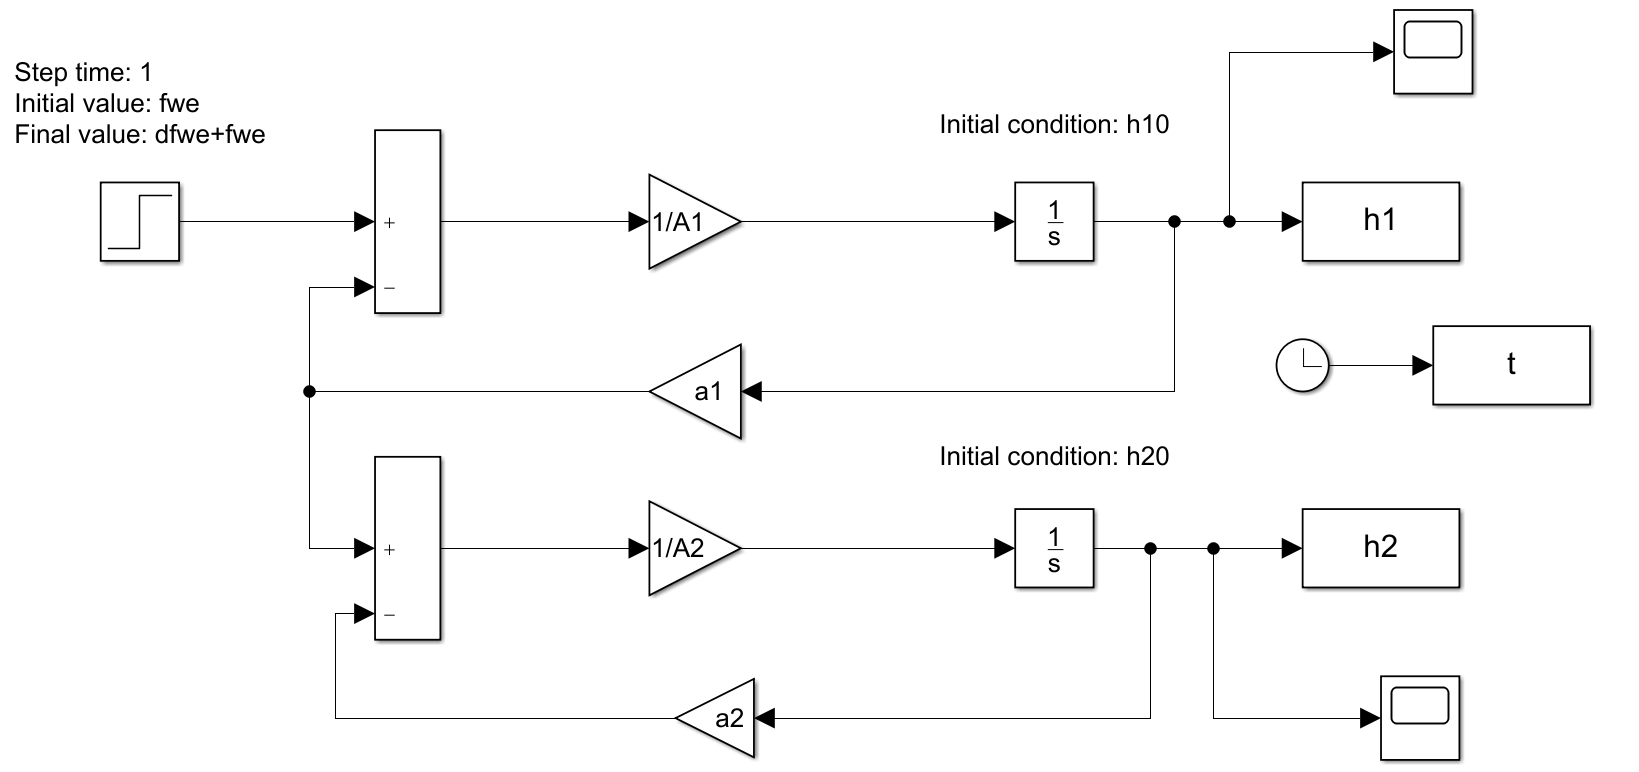
\includegraphics[width=1\textwidth]{schematL.png}
    \label{fig:my_label}
\end{figure}
\section{Odpowiedzi skokowe.}
 $$df_{we}=10\% \cdot f_{we max}$$
 a)$fwe=0$\\
 dla modelu nieliniowego:
 \begin{figure}[h!]
    \centering
    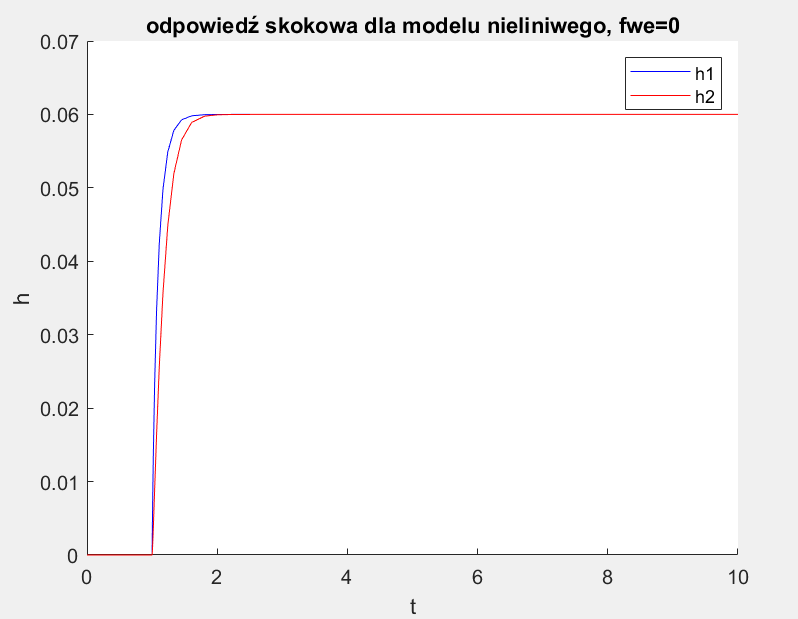
\includegraphics[width=0.6\textwidth]{skokNL0.png}
    \label{fig:my_label}
\end{figure}
\newpage
dla modelu liniowego:
\begin{figure}[h!]
    \centering
    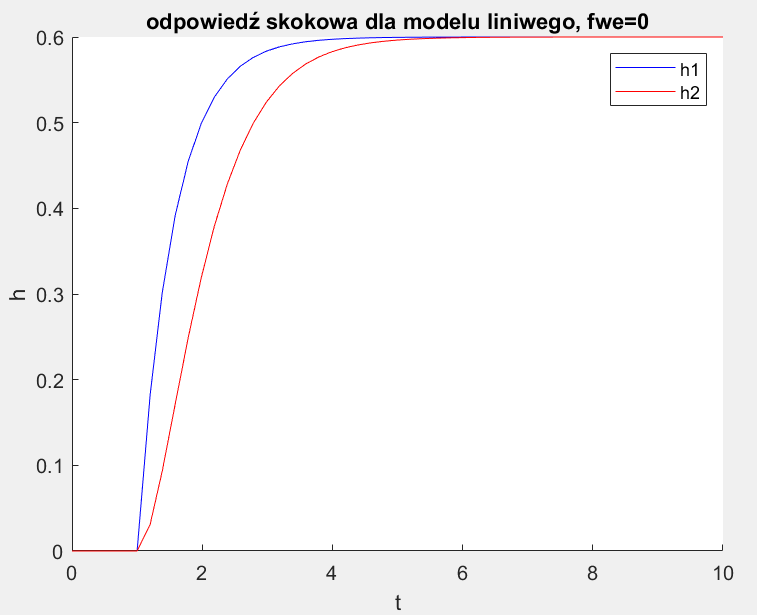
\includegraphics[width=0.6\textwidth]{skokL0.png}
    \label{fig:my_label}
\end{figure}
\begin{flushleft}
b)$fwe=0,5\cdot fwe_{max}$\\
 dla modelu nieliniowego:
\end{flushleft}
 
 \begin{figure}[h!]
    \centering
    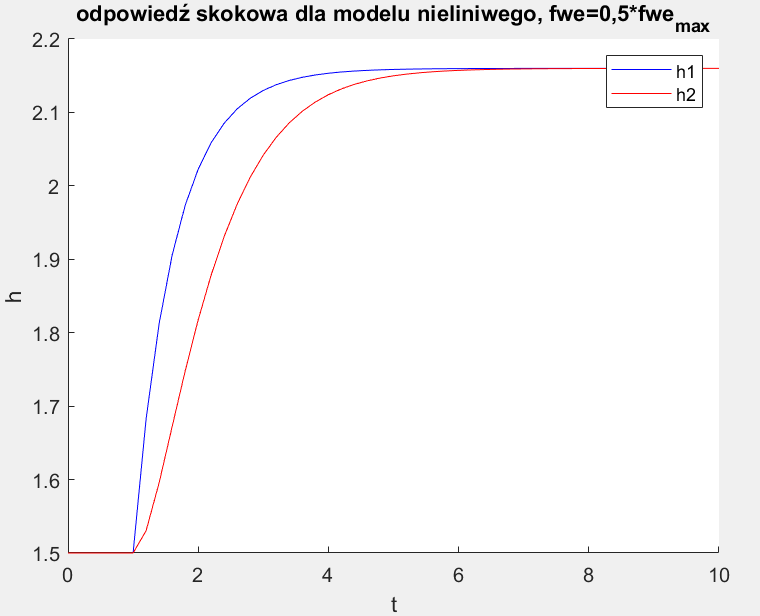
\includegraphics[width=0.6\textwidth]{skokNL05.png}
    \label{fig:my_label}
\end{figure}
\newpage
\begin{flushleft}
dla modelu liniowego:
\end{flushleft}

\begin{figure}[h!]
    \centering
    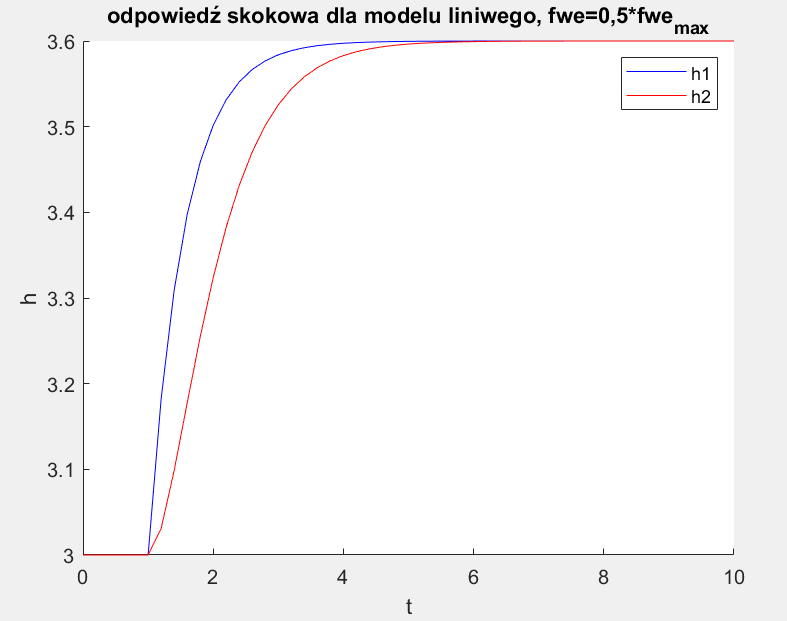
\includegraphics[width=0.6\textwidth]{skokL05.png}
    \label{fig:my_label}
\end{figure}
\begin{flushleft}
c)$fwe=0,9 \cdot fwe_{max}$ \\
dla modelu nieliniowego:
\end{flushleft}


 \begin{figure}[h!]
    \centering
    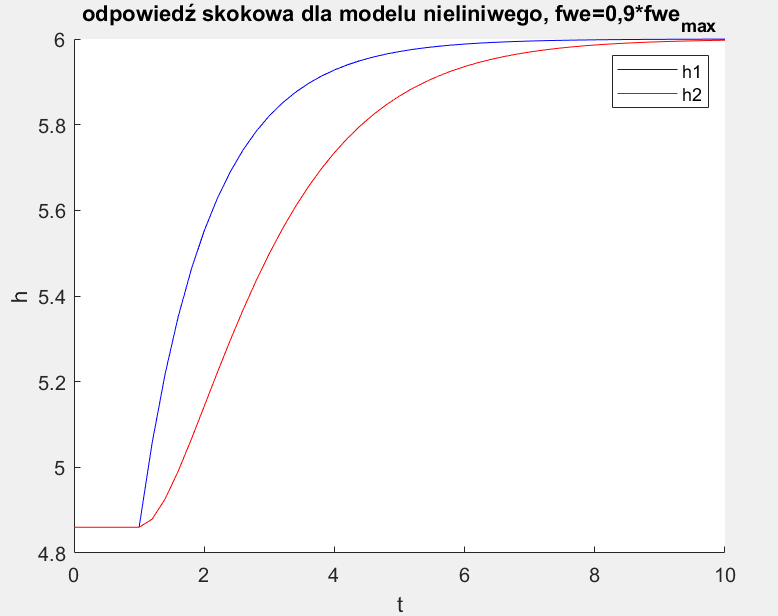
\includegraphics[width=0.6\textwidth]{skokNL09.png}
    \label{fig:my_label}
\end{figure}
\newpage
\begin{flushleft}
dla modelu liniowego:
\end{flushleft}

\begin{figure}[h!]
    \centering
    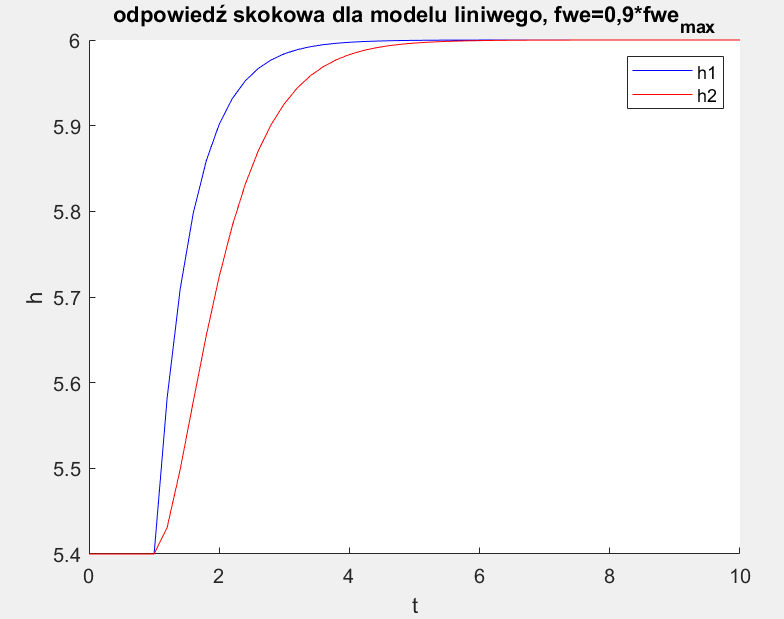
\includegraphics[width=0.6\textwidth]{skokL09.png}
    \label{fig:my_label}
\end{figure}
\section{Wnioski.}
Wykresy odpowiedzi skokowej dla modeli liniowych i nieliniowych różnią się w od siebie. W modelu nieliniowym wraz ze zmianą skoku zmienia się zarówno wartość na której układ się ustabilizuje jak i czas w którym do tego dochodzi, w modelu liniowym wraz ze zminą skoku zamianie ulega tylko wartość na któej układ się ustabilizuje. 
\section{Załącznik.}
\begin{figure}[h!]
    \centering
    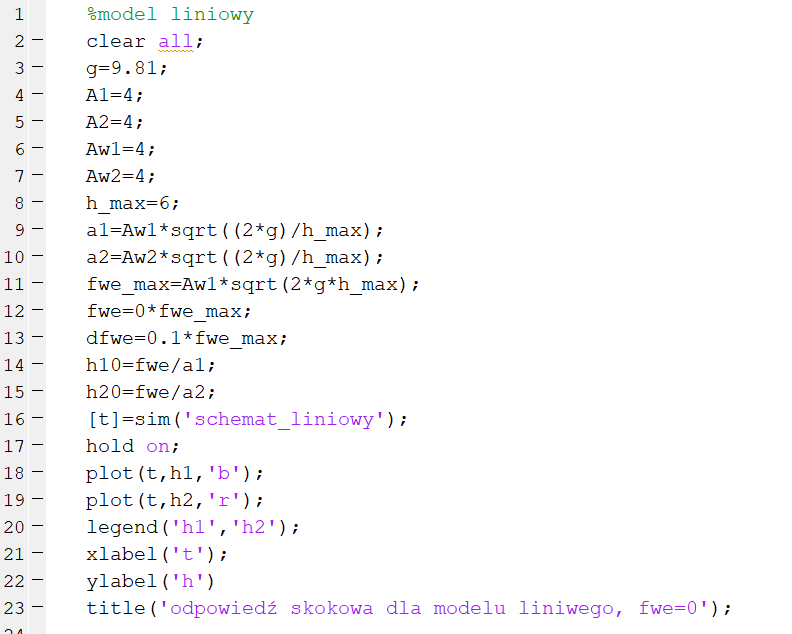
\includegraphics[width=0.6\textwidth]{kod1.png}
    \label{fig:my_label}
\end{figure}
\begin{figure}[h!]
    \centering
    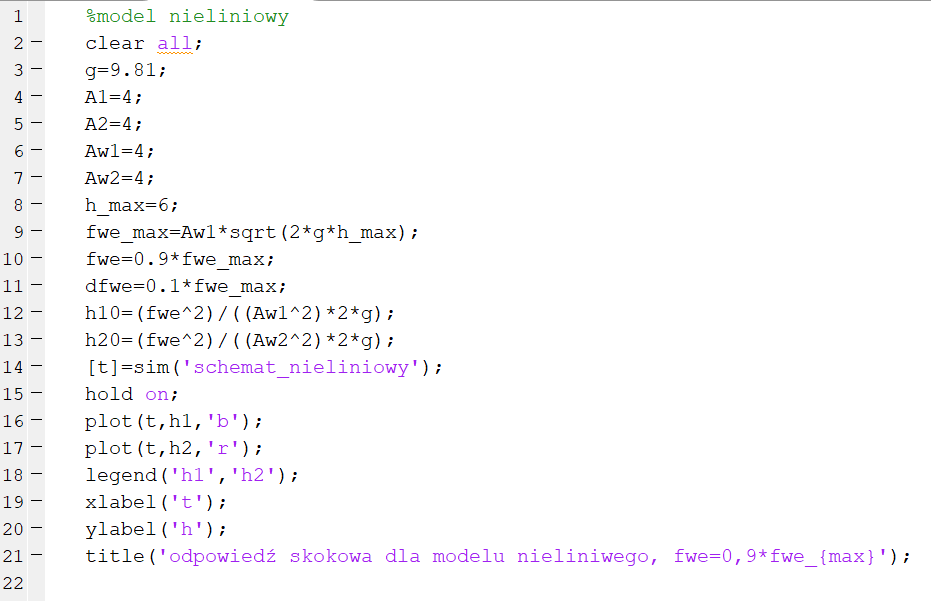
\includegraphics[width=0.6\textwidth]{kod2.png}
    \label{fig:my_label}
\end{figure}
\end{document}
